\documentclass{article}[12pt]
%Required: You must have these
\usepackage{graphicx}
\usepackage{tabularx}
\usepackage{natbib}
\usepackage{caption}
\usepackage{subcaption}
\usepackage{array}
\usepackage{amsmath}
\usepackage{amsfonts}
\newcommand{\overbar}[1]{\mkern 1.5mu\overline{\mkern-15mu#1\mkern-15mu}\mkern 1.5mu}

%\usepackage[backend=bibtex]{biblatex}
\setkeys{Gin}{width=0.8\textwidth}
%\setlength{\captionmargin}{30pt}
\setlength{\abovecaptionskip}{10pt}
\setlength{\belowcaptionskip}{10pt}
\topmargin -1.5cm 
\oddsidemargin -0.04cm 
\evensidemargin -0.04cm 
\textwidth 16.59cm
\textheight 23.94cm 
\parskip 7.2pt 
\renewcommand{\baselinestretch}{1.5} 	
\parindent 0pt

\bibliographystyle{refs/styles/newphyto.bst}
\usepackage{xr}
%\usepackage{hyperref}

\externaldocument{suppliment}
\externaldocument{prunus_nphyt_revresp_partI}

\usepackage{lineno}
\linenumbers
\title{Ecological drivers of flower-leaf sequences: aridity and pollination success select for flowering-first in the American Plums}  

\author{D.M. Buonaiuto $^{1,2,3,a}$, T.J. Davies $^{4,5}$, S. Collins $^{4}$ \& E.M. Wolkovich$^{2,3,4}$}
\date{}
\usepackage{Sweave}
\begin{document}
\input{3plums_new_phyt_revisionsJan2024-concordance}
\maketitle
 \noindent \emph{Author affiliations:}\\
\noindent $^1$Department of Environmental Conservation, University of Massachusetts, Amherst, Massachusetts, USA. ORCID: 0000-0003-4022-2591\\
\noindent 
$^2$Arnold Arboretum of Harvard University, Boston, Massachusetts, USA.\\
$^3$Department of Organismic and Evolutionary Biology, Harvard University, Cambridge, Massachusetts, USA \\
$^4$Forest \& Conservation Sciences, Faculty of Forestry, University of British Columbia, Vancouver, British Columbia, Canada\\
$^5$ Department of Botany, University of British Columbia, Vancouver, British Columbia, Canada\\
$^a$Corresponding author: 617.823.0687; dbuonaiuto@umass.edu\\

Word Count: Introduction 944:, Materials and Methods: 1722, Results: 501, Discussion:1394, \textbf{Total: 4561}
Figures: 4\\

\pagebreak

\section*{Summary} %lang for new phyt\
\begin{itemize}
\item Across temperate forests many tree species produce flowers before their leaves emerge. This flower-leaf phenological sequence, known as hysteranthy, is generally described as an adaptation for wind-pollination. However, this explanation does not address why hysteranthy is also common in biotically-pollinated taxa.

\item We quantified flower-leaf sequence variation in the American plums (\emph{Prunus}, subspp. \emph{Prunus} sect. \emph{Prunocerasus}), a clade of insect-pollinated trees, using herbaria specimens and Bayesian hierarchical modeling. We tested two common, but rarely interrogated hypotheses---that hysteranthy confers aridity tolerance and/or pollinator visibility---by modeling the associations between hysteranthy and related traits. To understand how these phenology-trait associations were sensitive to taxonomic scale and flower-leaf sequence classification, we then extended these analyses to all \emph{Prunus} species in North America. 

\item Our findings across two taxonomic levels support the hypotheses that hysteranthy may help temporally partition hydraulic demand to reduce water stress, and increase pollinator visibility and thereby reduce selective pressure on inflorescence size.


\item Our results provide foundational insights into the evolution of flower-leaf sequences in the genus \emph{Prunus}, with implications for understanding these patterns in biotically-pollinated plants in general. Our approach suggests a path to advance these hypotheses to other clades, but teasing out drivers fully will require new experiments.
\end{itemize}

Keywords: Deciduous forests, Flower-leaf sequences, Hysteranthy, Phenology, Plant hydraulics, Pollination, Phylogeny

\pagebreak
\section*{Introduction}
%<<label=numbers, echo=FALSE, results=hide, message=FALSE>>=
%rm(list=ls()) 
%options(stringsAsFactors = FALSE)
%require(brms,quietly = TRUE)
%setwd("~/Documents/git/proterant/investment/Input")
%load("pcerasus.Rda")
%doyeff<-round(fixef(mod.ord.scale.phlyo)[6],digits=2)
%doyints<-round(fixef(mod.ord.scale.phlyo)[6,3:4],digits=3)
\noindent Woody perennials\linelabel{uniq1} are among a subset of plant types with the unique ability to seasonally begin reproduction prior to vegetative growth. This flowering-first phenological sequence, known as hysteranthy, proteranthy or precocious flowering, is apparent in temperate deciduous forests around the globe \citep{Rathcke_1985}. A number of studies suggest that this flower-leaf sequence is under selection, and that hysteranthy can confer performance advantages \citep{Guo2014,Gougherty2018,Buonaiuto2020}, but the importance of variation in flower-leaf sequences for maintaining fitness may vary across functional types, taxa and biomes. %With mounting evidence that anthropogenic climate change is driving shifts in flower-leaf sequences \citep{Ma:2021tf,Wang:2022wt}, expanding our understanding of the adaptive benefit of hysteranthy may be important to forecasting the demography and performance of forest communities.

\noindent The most common, and well-tested explanation for the evolution of hysteranthy in temperate forests is that it is adaptive for wind-pollination, as leafless canopies increase wind speeds for pollen transport and reduce the likelihood of pollen interception by vegetation \citep{Whitehead1969,Niklas1985}. However, this explanation does not address the widespread prevalence of hysteranthy in biotically-pollinated taxa found in temperate regions. This number is not trivial; a recent analysis found that approximately 20\% of the hysteranthy species in Eastern Temperate Forests of North America are biotically-pollinated \citep{Buonaiuto2020}. 

Alternative hypotheses have been put forward to explain the advantage of hysteranthy in biotically-pollinated species, but they have not been widely evaluated in the literature. Below, we briefly review these hypotheses and their predictions, then test their predictions using the American plums (\textit{Prunus} subspp. \textit{Prunus} sect. \textit{Prunocerasus})---a widespread clade with high variability in flower-leaf sequences, as a case-study. Our study both clarifies the hypothesized function of flower-leaf sequence variation in the genus \emph{Prunus} and lays the groundwork for understanding the origins of flower-leaf sequence variation in biotically-pollinated taxa more generally.

\subsection*{Hypotheses of hysteranthous flowering in biotically-pollinated taxa}

\underline{Water limitation hypothesis:} In the dry-deciduous tropics of South and Central America, hysteranthy is common \citep{Rathcke_1985,Franklin2016}, and is regarded as an important adaptation to alleviate water stress by partitioning the hydraulic demand of flowers and leaves across the season \citep{Borchert1983,Reich1984,Franklin2016,Gougherty2018}. Under this hypothesis, the function of hysteranthous flowering in temperate regions parallels that in the dry tropics. While temperate forests are rarely water-limited in the early season during which flowering and leafing occur \citep{Polgar2011}, there is still considerable variation in water availability in space and time within temperate regions of the globe.  With this hypothesis, we would expect to find hysteranthous taxa in locations that are, on average, drier than their non-hysteranthous relatives.

\underline{Insect visibility hypothesis:} Hysteranthous flowers are visually conspicuous in the landscape. Thus, as in wind-pollinated taxa, hysteranthy in biotically-pollinated taxa may be an adaptation for pollination efficiency as flowering-first species are easier for insect pollinators to locate \citep{Janzen1967}. A challenge\linelabel{caveat1} to evaluating this hypothesis is that correlated selection between flower-leaf sequences and pollinator visibility could have either a positive or negative relationship depending on the pollination environment. In one scenario, hysteranthy may be associated with smaller floral displays: because flowers are not obscured by leaves, they are easier to see and there is weaker selection for increasing floral display size. In an alternative scenario, hysteranthy could be associated with larger floral displays, especially in environments where plants are more often pollen-limited and selection may favor both hysteranthy and increased floral display size to augment floral attraction to visual\linelabel{caveat2} pollinators.
%\underline{Fruit maturaturion hypothesis:} There are several aspects of reproductive development that suggest hysteranthy is a by-product of developmental constraints related to fruit maturation. Hysteranthy may be common in large fruited species that require lots of time to mature their fruits, or in small, early fruiting species that have evolved dispersal syndromes (wind dispersal, non-dormant seeds) that require dispersal early in the season \citep{Primack1987}. In either case, we should expect fruit size to associate with hysteranthy, although the sign of the correlation differs.

In contrast to these functional hypotheses, hysteranthous flowering could simply be a by-product of selection for early flowering. Species that flower before their leaves inherently flower early in the season. For\linelabel{null1} example, fruit development or dispersal constraints may drive early flowering \citep{Primack1987}, and because spring flower phenology is less constrained by prior phenological events than leaf phenology \citep{Ettinger2018,Savage2019}, this selection for early flowering could incidentally produce the hysteranthous phenological sequence. Here, there is no specific adaptive advantage to hysteranthy;  selection is not operating on the relative timing of flower and leaf emergence, but rather the absolute flowering time alone. Rejection of the above functional hypotheses might provide support to this null explanation. 

\noindent A significant challenge for robust testing of hysteranthy hypotheses is that most characterizations of flower-leaf phenological sequences are based on expert-opinion verbal descriptions (e.g. ``flowers before leaves" or ``flower before/with leaves"), which make comparisons across taxa, time and space difficult and sensitive to observer bias  \citep[see][]{Buonaiuto2020}. This problem can be overcome by adopting standardized quantitative measures of plant phenology for observational studies and applying them to historical data records. Herbarium records are an excellent source of data that can be leveraged for quantitative phenological measurements \citep{Willis2017}, but have not been widely used to investigate variability of flower-leaf sequences.

\noindent The American plums %	(Genus: \emph{Prunus},	subspp. \emph{Prunus}	sect.	\emph{Prunocerasus}) 
are useful model clade to investigate drivers of hysteranthous flowering in biotically-pollinated species. The species that make up this group are distributed across the temperate zone of North America and, like the genus \textit{Prunus} more generally show pronounced inter-specific variation in flower-leaf sequences. Usefully, species in this clade are well represented in herbaria records (Fig. \ref{fig:phylo2}a), making them a tractable group to measure and assess variation in flower-leaf sequences.

\noindent To interrogate the functional hypotheses for hysteranthous flowering described above, we used herbaria records to quantify variation in flower-leaf sequences of the American plums. Then we combined environmental attributes, biological traits and phylogenetic data in statistical models designed to evaluate whether the observed associations between flower-leaf sequences and morphological and environmental traits match the predicted associations of the hysteranthy hypotheses. Finally, we compared our findings in this clade to patterns observed in larger genus \emph{Prunus} to test whether these phenology-trait associations were sensitive to taxonomic scale and flower-leaf sequence classification.

\section*{Materials and Methods}
\subsection*{Quantifying flower-leaf sequence variation}  
We obtained digital herbarium specimens of the American plums from the Consortium of Midwest Herbaria (CMH) Database \citep{CMH}. Specimen\linelabel{range1} collection dates ranged from 1844-2020, with the majority collected between\linelabel{range2} 1950-2000. To quantify flower-leaf sequence variation in this group we randomly sampled 200 specimens for each species and scored the phenological development of flowers and leaves; we used a modified BBCH scale for woody plants \linelabel{bbch1} designed to evaluate vegetative and reproductive phenological progress through a standardized quantitative index \citep{Finn2007}. For\linelabel{samps1} species with less than 200 specimens in the collection, we included all available specimens. In total, we evaluated the phenology of 2521 specimens, but only specimens with visible flowers were included in this analysis. We also removed specimens with flowering dates that were major outliers from the observed flowering period of each species. We removed outliers visually, and by excluding observations that were beyond three standard deviations of the median flowering time for each species ($n$=9). Our final analyses included 1000 specimens\linelabel{samps2} (see Tab. \ref{tab:samps} for number of observations/species). 

We reconstructed the phylogenetic relationships among species in this group based on the tree topology in \citet{Shaw:2004aa}. We inferred branch lengths following the method of \citet{Granfen1989} in which node heights are estimated in proportion to number of subtending taxa using the R package ``ape" \citep{Paradis2019}.

To quantify flower-leaf sequence variation, we fit an ordinal, hierarchical, Bayesian phylogenetic mixed model \citep{Garamszegi2014} designed to assess the likelihood an individual would be at any given vegetative BBCH phase while flowering. Our model predicted leaf stage ($y_i$, ordinal, with six categories representing stage from 1 for ``buds closed" and 6 for ``leaf expansion complete") as a function of species and additional phylogenetic effects. Because hysteranthy\linelabel{fiver} co-varies with flowering time (i.e., flowering first species will generally flower earlier than other species, on average), and collection\linelabel{bias1} dates were not evenly distributed across the flowering season (see Fig. \ref{fig:bias}), we included day of year of observation as an additional predictor. Additionally, because\linelabel{hinge1} climate change could affect the interval between flowering and leafout over the course of our time series, we included the year of collection of each specimen as a covariate. Following previous conventions for modeling the possible effects of climate change on spring phenology, we parameterized \emph{year} as a hinge variable, using 1980 as a break\linelabel{hinge2} point \citep{IPCC2013,Buonaiuto2020}. 

The model is written below:\\

$y_i$ = \left\{ \begin{array}{lll}
1 & if & z_i < 0\\ 
2 & if & z_i  \in (0,c_{2})\\ 
3 & if & z_i \in (c_{2},c_{3})\\ 
4 & if & z_i \in (c_{3},c_{4})\\ 
5 & if & z_i \in (c_{4},c_{5})\\ 
6 & if & z_i > c_{5}\\ 
\end{array}\right.
\\

$z_i  &= \alpha+ \alpha_{phylo}+ \alpha_{sp}+ \beta_{\text{day of year[sp]}}*X_{\text{day of year}}+ \beta_{year}*X_{year}+ \epsilon_i$\\
  
$\epsilon_i & \sim logistic(0,1)$ \\ 
   
where $y_i$ is the ordinal outcome (leaf stage; as 1,2,...6 categories). $c_{2...5}$ are the estimated cutpoints between leaf stages on the logit scale and $year$ is: (the year the specimen was collected $-$ 1980). $z_i$ is the linear component of the underlying latent variable model.  

$\alpha$ describes an intercept for each category [1,2,...6] and slopes ($\beta_{\text{day of year}}}$ and $\beta_{year_}$) are constant across cutpoints. $\beta_{\text{day of year}}$ also varies among $species$ while $\beta_{year_}$ is a pooled estimate across species. 
  
  \noindent The influence of the phylogeny ($\alpha_{phylo}$) was modeled as:\\
  
  \alpha_{phylo} & \sim \text{normal}(0, COR[\sigma^2_{phylo}]) 
  
  \noindent The $\alpha$ for species effects independent of the phylogeny was modeled as:\\
  
 \alpha_{sp} & \sim \text{normal}(0, \sigma^2_{species}) \\ 

We used\linelabel{conty1} our model to predict the probability that each species would be observed at a given vegetative BBCH stage during flowering for each day of the flowering period of each species by extracting 1000 random draws from the posterior distribution. Next, for each day of the flowering season, we summed the predicted likelihood that species would be at BBCH 0  (``bud closed"), BBCH 07/09 (``bud break") or BBCH 11 (``start of leaf unfolding) vs. BBCH 15 (``leaf unfolding"), BBCH 17(``most leaves unfolded"), BBCH 19 (``leaf expansion complete")---this allowed us to quantify the likelihood that a species would be hysteranthous or non-hysteranthy respectively for each day of the season. We chose the BBCH 11/BBCH 15 boundary to define hysteranthous flowering because this is the earliest point in development when most leaves are unfurled enough to visually obscure flowers and transpire. Finally, we used these estimates to develop a flower-leaf sequence index: for this, we summed the likelihood of hysteranthy vs. non-hysteranthy across the full flowering period of each species, with 0 being never hysteranthous and 1 being always\linelabel{conty2} hysteranthous. To evaluate the sensitivity of our model to choice of cutoff, we also calculated a hysteranthy index using an alternative cutoff at the BBCH 09/BBCH 11, which did not alter the species' ranks on the index (see Tab. \ref{tab:mod1comps}).

To\linelabel{noday} better understand how within-season dynamics affected our inference, we also refit our model excluding \emph{day of year} as a predictor. This version of the model did not substantially alter the species' ranks on the index or our inference about the relationships between flower-leaf sequence variation and the trait representing the main hysteranthy hypotheses\linelabel{noday2} (Tab. \ref{tab:mod1comps}, Tab. \ref{tab:nodoy}). 

\subsection*{Evaluating hysteranthy hypotheses}
To test the hypotheses of hysteranthy, we first recorded petal length measurements directly from herbarium specimens. For these morphological measurements, we sampled 321 specimens and measured the petal length of up to 10 randomly selected petals per specimen ($n$=2757) using ImageJ image processing software (see Tab. \ref{tab:mod1comps}, for $n$ per species).% We also used ImageJ to measure the diameter of fruits on an additional 316 specimens, measuring up to 5 fruit per specimen (n=224).

To assess aridity tolerance, we computed the average Palmer\linelabel{pdsi1} Modified Drought Index score (hereafter: PDSI), obtained from the \citet{NOAA} for every \textit{Prunocerasus} specimen in the database ($n$=2305, see Tab. \ref{tab:mod1comps}, for $n$ per species). PDSI is a standardized index that integrates temperature and precipitation data to estimate relative dryness in time and\linelabel{pdsi2} space \citep{Heim:2002uw}. For any specimens that lacked accurate geo-location information, we extracted PDSI values at the county centroid of the herbaria specimen. 

Because\linelabel{just1} all of our measurements were made on different individuals---with different sample sizes---we used two different modeling approaches to test the relationship between flower-leaf sequence index scores, aridity tolerance and floral\linelabel{just2} displays.

First we computed species-level means of PDSI and petal length and used a beta regression to evaluate the relationship between flower-leaf sequences, PDSI, petal length and their interaction. We standardized the units of all predictors through $z$-scoring \citep{Gelman2007} to make their effect size estimates directly comparable within the following model structure:\\

$y_i = (\mu,\mu(1-\mu)/(1+\phi)$\\

where $\mu$ and $\phi$ are the two shape parameters of the beta regression. Due to the limited sample size of this analysis (13 species), we only modeled the effect of our predictors on the mean parameter $\mu$ and fit a grand intercept for the precision parameter $\phi$.We modeled the $\mu$ parameter as: \\

$\mu = \alpha+ \beta_{PDSI}*{\overline{X_{PDSI}}+\beta_{\text{petal length}}*\overline{X_{\text{petal length}}}+\beta_{PDSI_x \text{petal length}}*(\overline{X_{PDSI}})(\overline{X_{\text{petal length}}})$\\
%
%$\phi = \alpha$\\

%https://cran.rstudio.com/web/packages/betareg/vignettes/betareg-ext.pdf

We chose this model structure because it allowed us to assess the additive and interactive effects of PDSI and petal size on flower-leaf sequences. However, by using mean trait values as predictors, we could not incorporate within-species variation in these trait/environmental predictors or account for their phylogenetic structure. To understand how these factors affected our inferences about the relationship between flower-leaf sequences and traits, we fit two additional models to estimate relationship between flower-leaf sequences index values and PDSI, and between flower-leaf sequences index values and petal size separately which included the intra-specific variation and phylogenetic structure of each of these traits (see Supporting Information: Extended Methods for details). This alternative modeling approach produced similar results about the phenology-trait relationships investigated in our main model.
%We also ran each model using our two alternative flower-leaf sequence indexing approaches to make sure our results were robust to choice of index. Though these alternative classification schemes did change the hysteranthy index score for some species (Fig. \ref{fig:plums}), they did not substantially impact the inference from our models (see Tab. \ref{tab:modput} for comparisons).
\subsection*{Hysteranthy in the larger genus \textit{Prunus}}
To better understand how the patterns we identified in the American Plums clade scaled across coarser taxonomic resolution, we also evaluated the relationship between hysteranthous flowering and hypothesis-related traits for additional \textit{Prunus} species native to, or established in, North America\linelabel{n1} ($n$=32). For this analysis, we obtained categorical descriptions of flower-leaf sequences and mean estimates of the number of flowers per inflorescence as a proxy for floral investment from the \underline{Flora of North America} \citep{Rohrer_1993}.  We extracted PDSI values for all herbaria observations of those species in the Consortium of Midwest Herbaria database ($n$=23,272) as described above.

To account for the influence of evolutionary relationships among species, we reconstructed the phylogenetic relationships in the genus based on the tree topology in \citet{Chin:2014wu}. As above, we computed branch lengths with the R package ``ape" \citep{Paradis2019}. 

As above, we standardized the units of all predictors through $z$-scoring \citep{Gelman2007}. The model structure is:
 

$y_i$ = \left\{ \begin{array}{lll}
1 & if & z_i < 0\\ 
2 & if & z_i  \in (0,c_{2})\\ 
3 & if & z_i \in (c_{2},c_{3})\\ 
4 & if & z_i> c_{3}\\ 
\end{array}\right.
\\

$z_i$ &= \alpha+ \alpha_{phylo}+ \beta_{PDSI}*X_{PDSI}+\beta_{\text{floral investment}}*X_{\text{flowers/inflorescence}}+\beta_{PDSI_x \text{floral investment}} (X_{PDSI})(X_\text{flowers/inflorescence})+\epsilon_i$\\

   \epsilon_i & \sim logistic(0,1) \\ 
  
where $y_i$ is the ordinal outcome of flower-leaf sequence category ( ``flowers after leaves"=1, ``flowers with leaves"=2, ``flowers before/with leaves"=3 and ``flowers before leaves"=4) and $c_{2...3}$ are the estimated cutpoints between categories on the logit scale. $z_i$ is the linear component of the underlying latent variable model. $\alpha$ describes a grand intercept, and we modeled the influence of phylogeny ($\alpha_{phylo}$) as above. Note\linelabel{catergories} that this model includes four ordinal categories while our model of the American Plums clade included six, due to the different underlying structures of the two datasets.

\subsection*{Model runs} 
We fit all models in the R package ``brms" \citep{Burkner2018} using weakly informative priors, and four chains.
For the models aimed at ``Quantifying flower-leaf sequence variation" and ``Evaluating hysteranthy hypotheses" in the American plums, we ran the models with a warm-up of 3000 iterations, and 4000, and 5000 sampling iterations respectively, for a total of 4000 and 8000 sampling iterations across all chains. For the ``Hysteranthy in the larger genus \textit{Prunus}" model, we used a warm up of 6,000 iterations and 8,000 sampling iterations for a total of 8000 sampling iterations to maximize the effective sampling size. Model fits were assessed with  $\hat{R}$ <1.01, high effective sample sizes, and no divergent transitions. We provide mean estimates with  uncertainty intervals in-text, and 50\% and 89\% intervals for all figures and tables.

\section*{Results}
\subsection*{Quantifying flower leaf sequences in the American plums}
We found substantial inter-specific differences in flower-leaf sequences within the American plums\linelabel{oneby} (Fig. \ref{fig:phylo2}b,\ref{fig:ordinals}a). Several species (\emph{P. mexicana}, \textit{P. umbellata}, \textit{P. angustifolia}, \textit{P. maritima} and \textit{P. gracilis}) were most likely to be hysteranthous for all---or most---of their flower period, while for others, (\textit{P. americana}, \textit{P. munsoniana}, \textit{P. alleghaniensis}, \textit{P. nigra}, \textit{P. hortulana}, \textit{P. texana} and \textit{P. rivularis}), hysteranthous flowering was only likely in the early part of their flowering session. One species, \emph{P. subcordata}, was unlikely to be hysteranthous at any point in its flowering period (Fig. \ref{fig:ordinals}a). These relative ranking of species' hysteranthy likelihoods were consistent with our alternative method for constructing the hysteranthy index (Tab. \ref{tab:mod1comps}, Fig. \ref{fig:nodoy}).


Across all species of American Plums, day of year increased the likelihood of flowering during a later vegetative phenological stage (Fig. \ref{fig:ordinals}b). Year of observation did not substantially impact the likelihood of hysteranthy for this taxonomic group (Fig. \ref{fig:ordinals}b).

 
\subsection*{Associations between hysteranthy and environmental and morphological traits}
In the American plums, predominately hysteranthous species had smaller flowers and occured in drier localities than species with more overlap between flowers and leaves (i.e., increased likelihood of hysteranthy was negatively associated with PDSI and petal length without a substantial interaction between them, Fig. \ref{fig:prunes}a, b; parameter estimates from this model were  $\beta_{PDSI}: -0.47, UI_{89}[-0.96, 0.01]$, $\beta_{\text{petal length}}: -0.14,UI_{89}[ -0.54, 0.24]$  $\beta_{PDSI_x \text{petal length}}: -0.14,UI_{89}[ -0.91, 0.65]$). These estimates were comparable to estimates from models where we treated each predictor separately and accounted for phylogeny (Fig. \ref{fig:seps}), and where we used the hysteranthy index derived from models that did not include day of year as a predictor (Tab. \ref{tab:nodoy}). The direction and magnitude of the estimated effects support the predictors of the water-limitation hypothesis and marginally support the predictors of the insect-visibility hypothesis. 

In the larger genus \emph{Prunus}, hysteranthous species had smaller inflorescences and were found in drier locations (i.e., there was a negative association between hysteranthy and PDSI and number of flowers per inflorescence, as well as a substantial negative interaction between them, Fig. \ref{fig:genus}a, b; parameter estimates from this model were  $\beta_{PDSI}:-8.0, UI_{89}[-16.6,-2.44]$,  $\beta_{flowers/inflorescence}: -15.5, UI_{89}[-31.46,-5.56]$ and $\beta_{PDSI x flowers/inflorescence}: -13.06, UI_{89}[-28.53,-2.93]$).  The direction and magnitude of the estimated effects support the predictors of both the water-limitation hypothesis and the insect-visibility hypothesis.

The estimated effects of floral traits and their interactions with PDSI were stronger in the larger genus \emph{Prunus} than in the American plums clade.
This is not\linelabel{floflo1} surprising given that all species in the American plums clade have solitary flowers, making the variation in floral display size highly constrained. By contrast, \emph{Prunus} species included in our secondary analysis include those with  solitary flowers and species with as many as 100 flowers per inflorescence---substantially more variation in both floral investment and in hydraulic demand. This suggests that the correlated selection between flower-leaf sequences and these floral traits may be more pronounced at coarser taxonomic resolutions, where underlying trait variation is\linelabel{floflo2} greater.

\section*{Discussion}
Using\linelabel{style1} North American \textit{Prunus} species as a case study, our analyses indicate that flower-leaf sequences are likely under selection. We show that variation in flower-leaf sequences across species may reflect adaptive tradeoffs between\linelabel{tradeoffz} a) the timing of investment in reproduction relative to the timing of resumption of carbon acquisition through leafout, and b) other aspects of plant performance, such as environmental tolerance and pollinator attraction strategies that we investigated in this study. We show that hysteranthous flowering is associated with increased aridity and smaller flower displays in both the American plums, and more broadly across \emph{Prunus} species native to, or established in North America. The relationships between hysteranthy and aridity, and hysteranthy and floral display size support the predictions of the water limitation hypothesis and the insect visibility\linelabel{style2} hypothesis. 

Our models estimated a strong relationship between aridity and flower-leaf sequences at both taxonomic scales we studied, but the relationship between floral display size and flower-leaf sequences predicted by the insect visibility was better supported at the coarser taxonomic scale of the full genus \emph{Prunus} than in the American Plums clade. This contrast may suggest that associated selection between flower-leaf sequences and pollinator traits has more strongly influenced inflorescence architecture than the morphology of individual flowers, our estimates at both scales agreed in directionality (i.e., hysteranthy associated with smaller floral displays). 

Under the insect visibility hypothesis, floral display size could either be positively or negatively associated with hysteranthy depending on the pollination environment. The association between hysteranthy and smaller flower displays we found supports the prediction that increased visibility of hysteranthous flowers reduces selection pressure on flower display size. These results fit with other comparative anatomy studies in plants that report hysteranthous species typically have smaller inflorescences than non-hysteranthous relatives \citep{Gunatilleke1984}, and studies on pollinator foraging behavior that suggest the presence of leaves substantially alters the visual perception of pollinators \citep{Rivest:2017aa,Forrest:2009aa}.% providing further evidence to refine the predictions of this hypothesis.

Our support for both the water limitation hypothesis and insect visibility hypothesis, and the strong positive interactions between PDSI and floral investment that we observed in the larger genus \emph{Prunus} highlight that these hypotheses are not mutually exclusive, and could be related. Selection on floral size represents a classic evolutionary tradeoff where larger floral displays may generally be more effective for attracting pollinators but demand more resources, including water, to maintain turgor and reproductive function than smaller ones \citep{Galen:1999vr,Lambrecht:2007ur}. With this trade-off, reproductive displays are often small in harsher environments \citep{Lambrecht:2013aa,Teixido:2016aa}, and hysteranthy could represent a compensatory mechanism that both reduces hydraulic demand while increasing pollination efficiency in these environments. %Studies that have compared the transpiration rates among flowers and leaves provide insights to the potential importance of this seasonal partitioning for maintaining water status. Measurements of water movement (transpiration rates, sap flow, hydraulic conductivity) to flowers range from 20\%-60\% of that of leaves under comparable conditions \citep{Whiley:1988uf,Roddy:2012wn,Liu:2017wg,McMann:2022ww}. This level of additional hydraulic demand can drive loss of stomatal conductance and decrease photosynthetic rates \citep{Galen:1999vr}.
 
Despite this evidence that hysteranthy can reduce hydraulic demand in dry environments, hysteranthous species in the American plum clade are not found in extremely arid locations (PDSI values typically range from -4 to 4, although the values that we observed in our analyses were more restricted, ranging from -0.5 to 0.2). This contrasts with hysteranthous species in the dry tropics where this phenological pattern appears to allow them to tolerate more extreme aridity \citep{Franklin2016}. But the flower-leaf sequences of the hysteranthous species in our study were markedly different from patterns of hysteranthy in these dry-tropics where the water limitation hypothesis was initially proposed. While flowering can precede leafout by as much several weeks for species in the American plums, the process of fruit development, which is also water intensive, occurs when leaves are present. By contrast, in the dry tropics hysteranthous flowering is initiated at the time of leaf drop \citep{Borchert1983,Franklin2016}; thus, the full reproductive cycle occurs in the leafless period. The comparatively small window of leafless reproductive development in our temperate clade may, in part, explain why the association we observed between hysteranthy and aridity was relatively weak and variable. Our results suggest that hysteranthy may allow temperate species to occupy marginally drier environments than non-hysteranthous species, but may not facilitate species' persistence under extreme aridity. 

\subsection*{Inter-and intra-specific variation in flower-leaf sequences} %emw -- also great first sentence below
We developed a novel approach to assessing flower-leaf sequences that scales from quantitative, individual-level observations to species-level characterizations. With this approach, we were able to---for the first time---quantitatively assess intermediate cases of hysteranthy (such as those that are typically described as ``flowers before/with leaves"). Previous studies of hysteranthous flowering have either excluded these cases from their analyses  \citep[e.g.;][]{Gougherty2018} or binned them with the well defined cases \citep[e.g.;][]{Buonaiuto2020}. We found that many American plum species expressed this intermediate flower-leaf sequence. Further, while our classifications broadly matched previous species-level analyses in this group by \citet{Shaw:2004aa}, our approach identified substantial differences in flower-leaf sequences among these intermediate cases (Fig. \ref{fig:phylo2}b), which allowed us to assess the trait associations with this phenotype.
%OLD We found that many American plum species expressed this intermediate flower-leaf sequence, and our classifications broadly matched previous species-level analyses in this group by \citet{Shaw:2004aa}. By estimating the likelihood of hysteranthy across the growing season with Bayesian methods, our approach identified substantial differences in flower-leaf sequences among these intermediate cases (Fig. \ref{fig:phylo2}b), which allowed us to assess the trait associations with this phenotype.
% 

Our quantitative analysis of the American plums clade revealed that flower-leaf sequences---often described as a species-level trait---are highly variable within species (Fig. \ref{fig:ordinals}a). For almost all members of the clade, hysteranthy was strongly predicted by the day of the observation (``day of year" in our model, Fig. \ref{fig:ordinals}b). In many cases there was a high likelihood that individuals of a species may be observed at different vegetative stages during flowering (Fig. \ref{fig:ordinals}a, Fig. \ref{fig:nodoy}). This variation could either suggest high levels of local adaptation in flower-leaf sequences or, alternatively, high levels of plasticity through which flower-leaf sequences respond to interannual variation in environmental conditions. Because\linelabel{lim1} our study was based on herbaria records collected on different individuals across space and time without repeat sampling, we could not robustly estimate how much flower-leaf sequences vary within vs. among species. However, this would be an important next step for understanding how the environment and species interactions have shaped these phenological\linelabel{lim2} patterns.

%emw22Oct -- below needs a little TLC, there's a lot of passive voice, jargon and some wordiness. 
%DB below is less relevant with the continuous indes
%By scoring these individual, quantitative observations as ordinal response categories with our hysteranthy index, we were able to contrast our findings to those derived from categorical, species-level characterizations based on expert opinion. The coherence between our individual based observational approach for the American plum clade and the top-down, categorical classification across \emph{Prunus} is an encouraging demonstration that the expert opinion-based data can still offer useful insights into the drivers of hysteranthous flowering when higher-resolution data is not available. 
 %emw22Oct -- below is good!
Interestingly\linelabel{climo1}, while there is substantial evidence that both flowering and leaf phenology have advanced over the last several decades in response to anthropogenic climate change \citep{Menzel2006,Cleland2007,Augspurger:2020aa}, we did not observe changes in flower-leaf sequences over that time scale in our dataset (Fig. \ref{fig:ordinals}b). This supports a recent finding that despite changes in both flowering and leafout, the time interval between them has remained relatively stable \citep{Guo:2023wb}, but does not preclude that possibility that these the sequences will eventually be disrupted as climate change continues to become more extreme\linelabel{climo2} in the future \citep{Buonaiuto_2021}.

\subsection*{Future directions}
We focused on a well-studied, and economically important clade of morphologically similar species. Our case-study provides a road map for evaluating the role of hysteranthy more generally in temperate biotically-pollinated plant taxa (other groups with high interspecific flower-leaf sequence variation include \emph{Magnolia}, \emph{Rhododendron}, \emph{Acer} and \emph{Cornus}), and more broadly across taxa and biomes.

Combining the observational approach with novel experiments could further advance our collective understanding of the adaptive significance of flower-leaf sequences. To test the water-limitation hypothesis, researchers could plant sister-taxa with contrasting flower-leaf sequences in common environments across a gradient of aridity, and evaluate their performance. To test the insect visibility hypothesis, researchers should consider hysteranthy---and phenology in general---in the broader framework of tradeoffs in pollination biology. The tradeoff between phenology and pollination investment could not only consider flower size, but also the number of flowers, nectar and pollen reward investment, volatiles between related hysteranthous and non-hysteranthous taxa. Findings that hysteranthous species invest fewer resources into these other pollinator attraction traits than non-hysteranthous relatives would support the insect visibility hypothesis. For a simple experiment to test the pollinator visibility hypothesis, researchers could force hysteranthy/non-hysteranthy phenotypes for the same genotype using environmental cues, and systematically release pollinators to observe their preferences, search times and foraging behavior. If pollinators are more readily drawn to the hysteranthous individuals, it would support hysteranthy as an adaptive trait for pollinator attraction. 

With a better mechanistic understanding of the relationship between flower-leaf sequences and ecological performance, researchers could then use experiments to assess how differences in floral and leaf physiological responses to temperature variation shape flower-leaf sequences. The measurement and modeling approaches we developed in our observational study can be readily implemented to analyze data from such experimental settings, presenting an important opportunity to unite observations of broad ecological patterns with targeted experimental manipulations to better understand both the evolutionary past and ecological future of flower-leaf sequences.


\section*{Competing Interests:}
The authors declare no conflict of interest.

\section*{Author contributions}
DMB, and EMW conceived of the manuscript; DMB and SC collected the data; DMB led the statistical analyses with TJD and EMW; DMB led the writing of the manuscript. All authors contributed to writing and gave approval for the submission.

\section*{Data Availability}
The phenology and trait data collected for this study will be made available and archived at KNB: The Knowledge Network for Biocomplexity (https://knb.ecoinformatics.org/) at the time of publication.

 %emw22Oct -- picky reviewers often complain about typos in the refs, I wonder if Sophia could help you here as you have a lot that need help ... though it is a latex-related annoyance so she may be less useful. 
\bibliography{refs/hyst_outline.bib} 

\newpage
\section*{Figures}


\begin{figure}[h!]
  \centering
 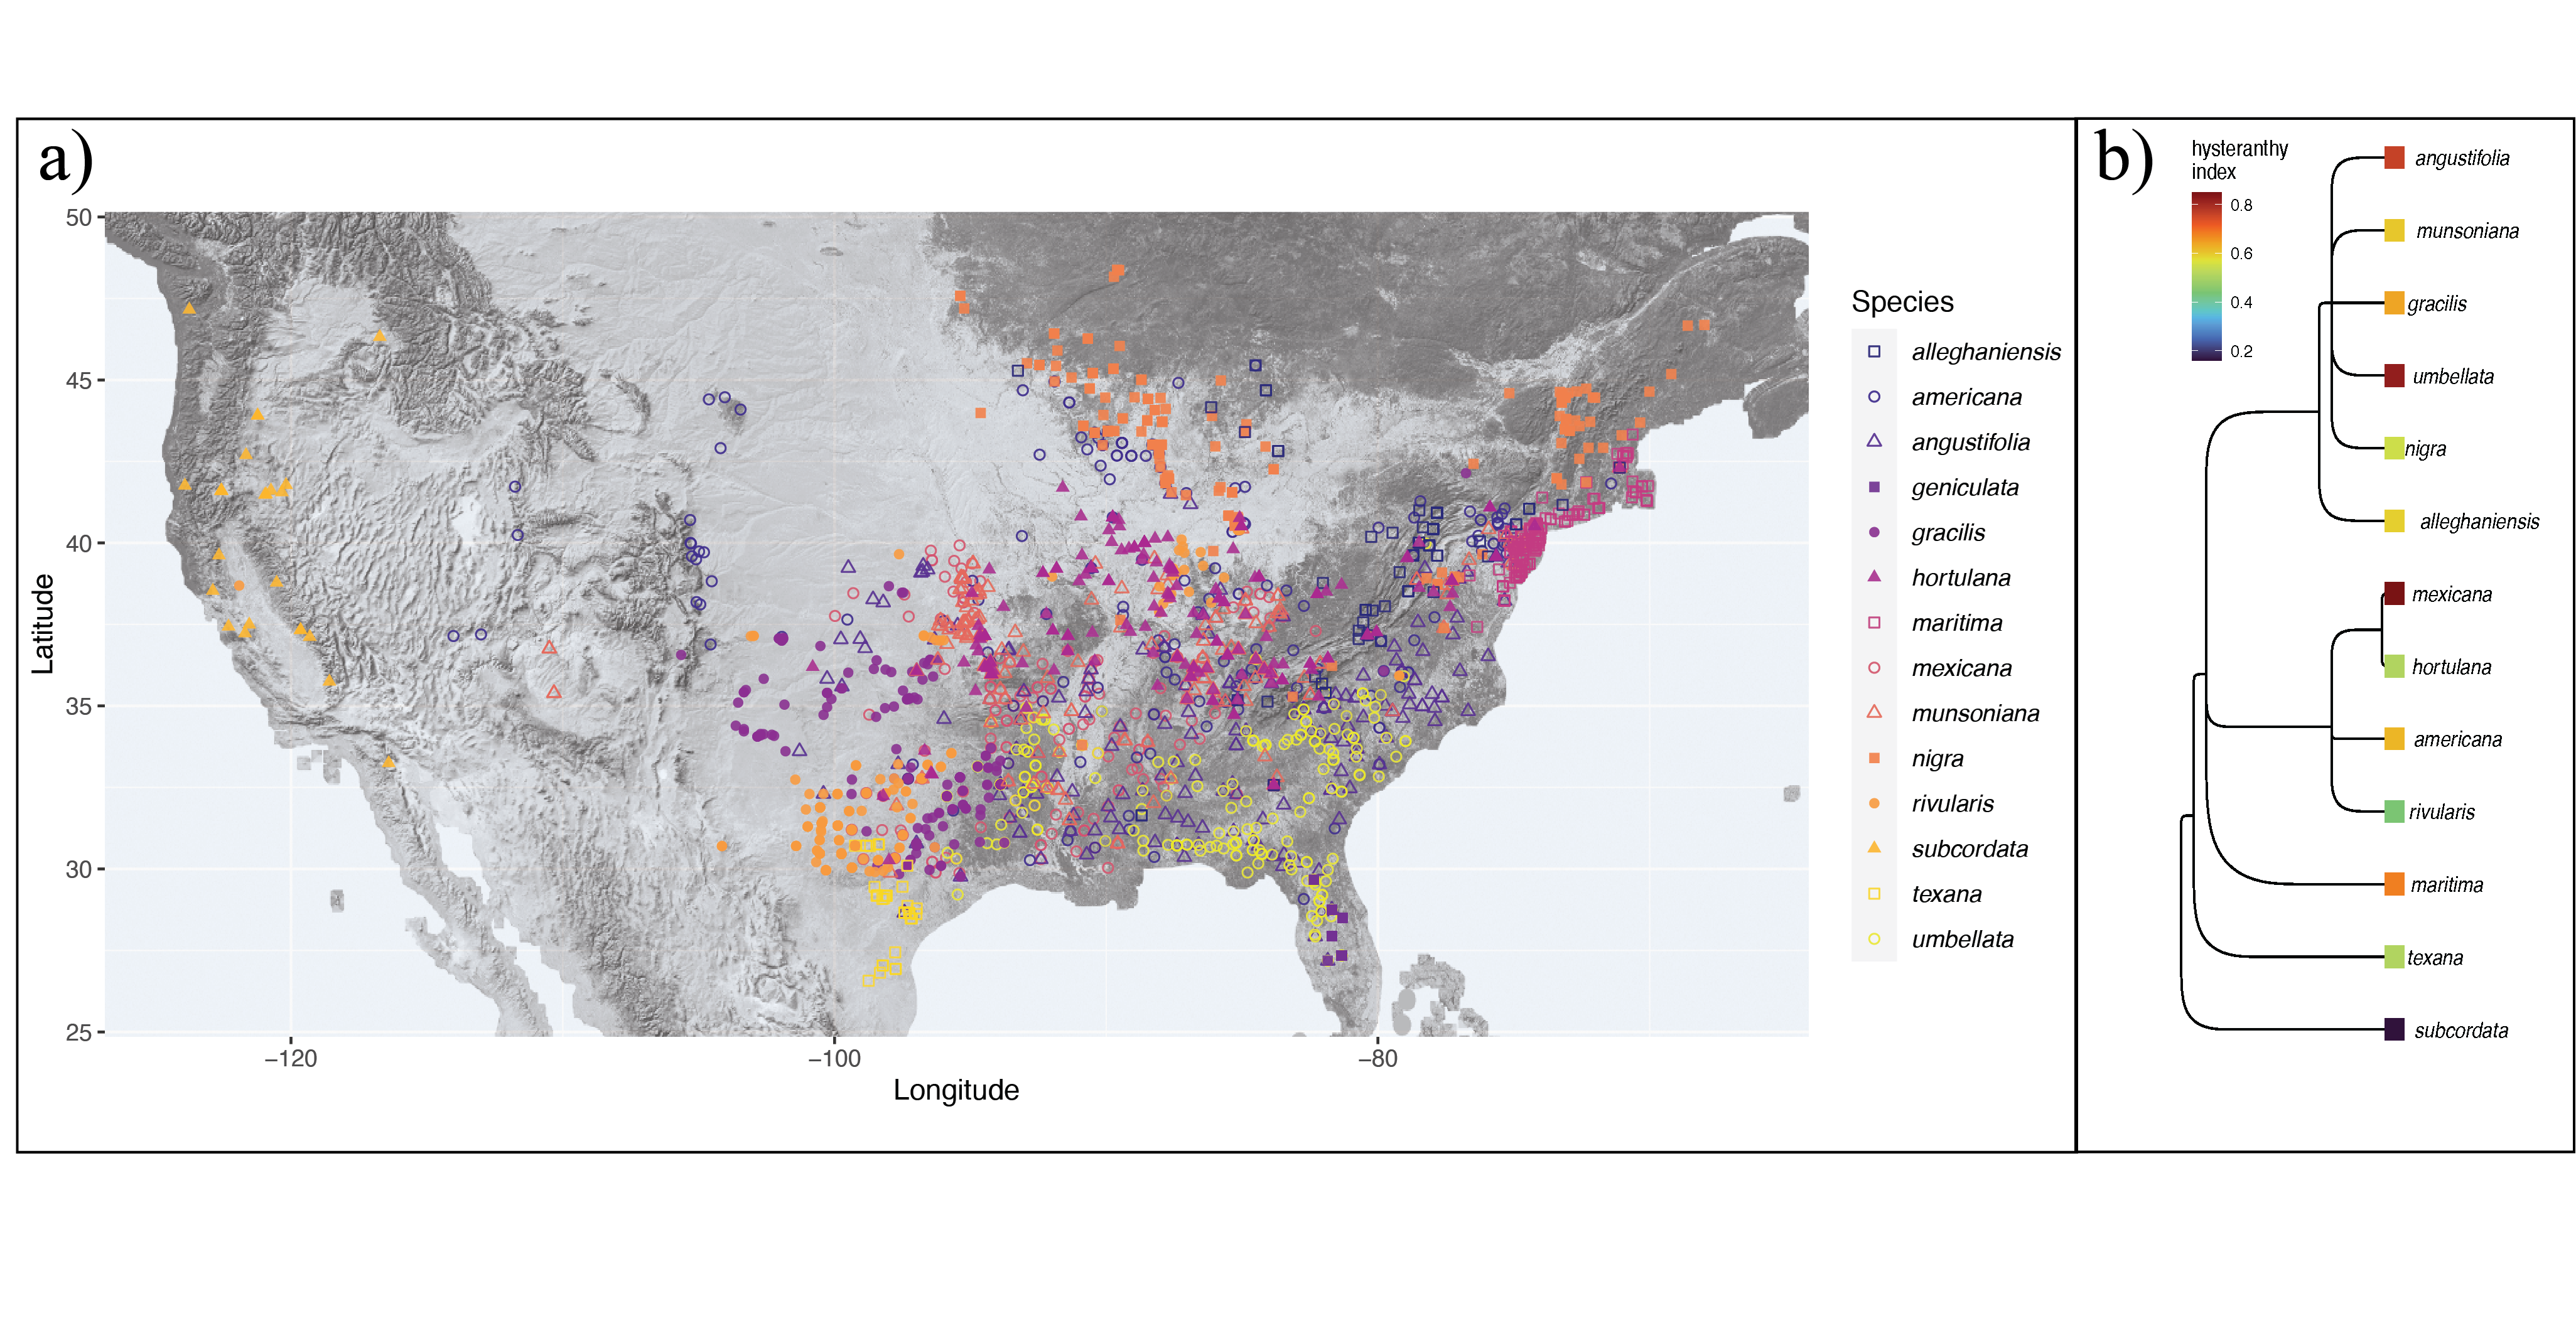
\includegraphics[width=\textwidth]{..//..//Plots/fig_1.png}
    \caption{Geographic distribution and taxonomic relationships among the American plums. a) Maps the localities of all the herbaria records used in this study. b) Depicts phylogenetic relationships among the American plums and the likelihood they each species is hysteranthous across its full flowering period, represented by a hysteranthy index where 0 is never hysteranthous and 1 is always hysteranthous. These designations are based on ordinal phylogenetic mixed models. Tree topology is from \citet{Shaw:2004aa}}
    \label{fig:phylo2}
\end{figure}



\begin{figure}[h!]
    \centering
 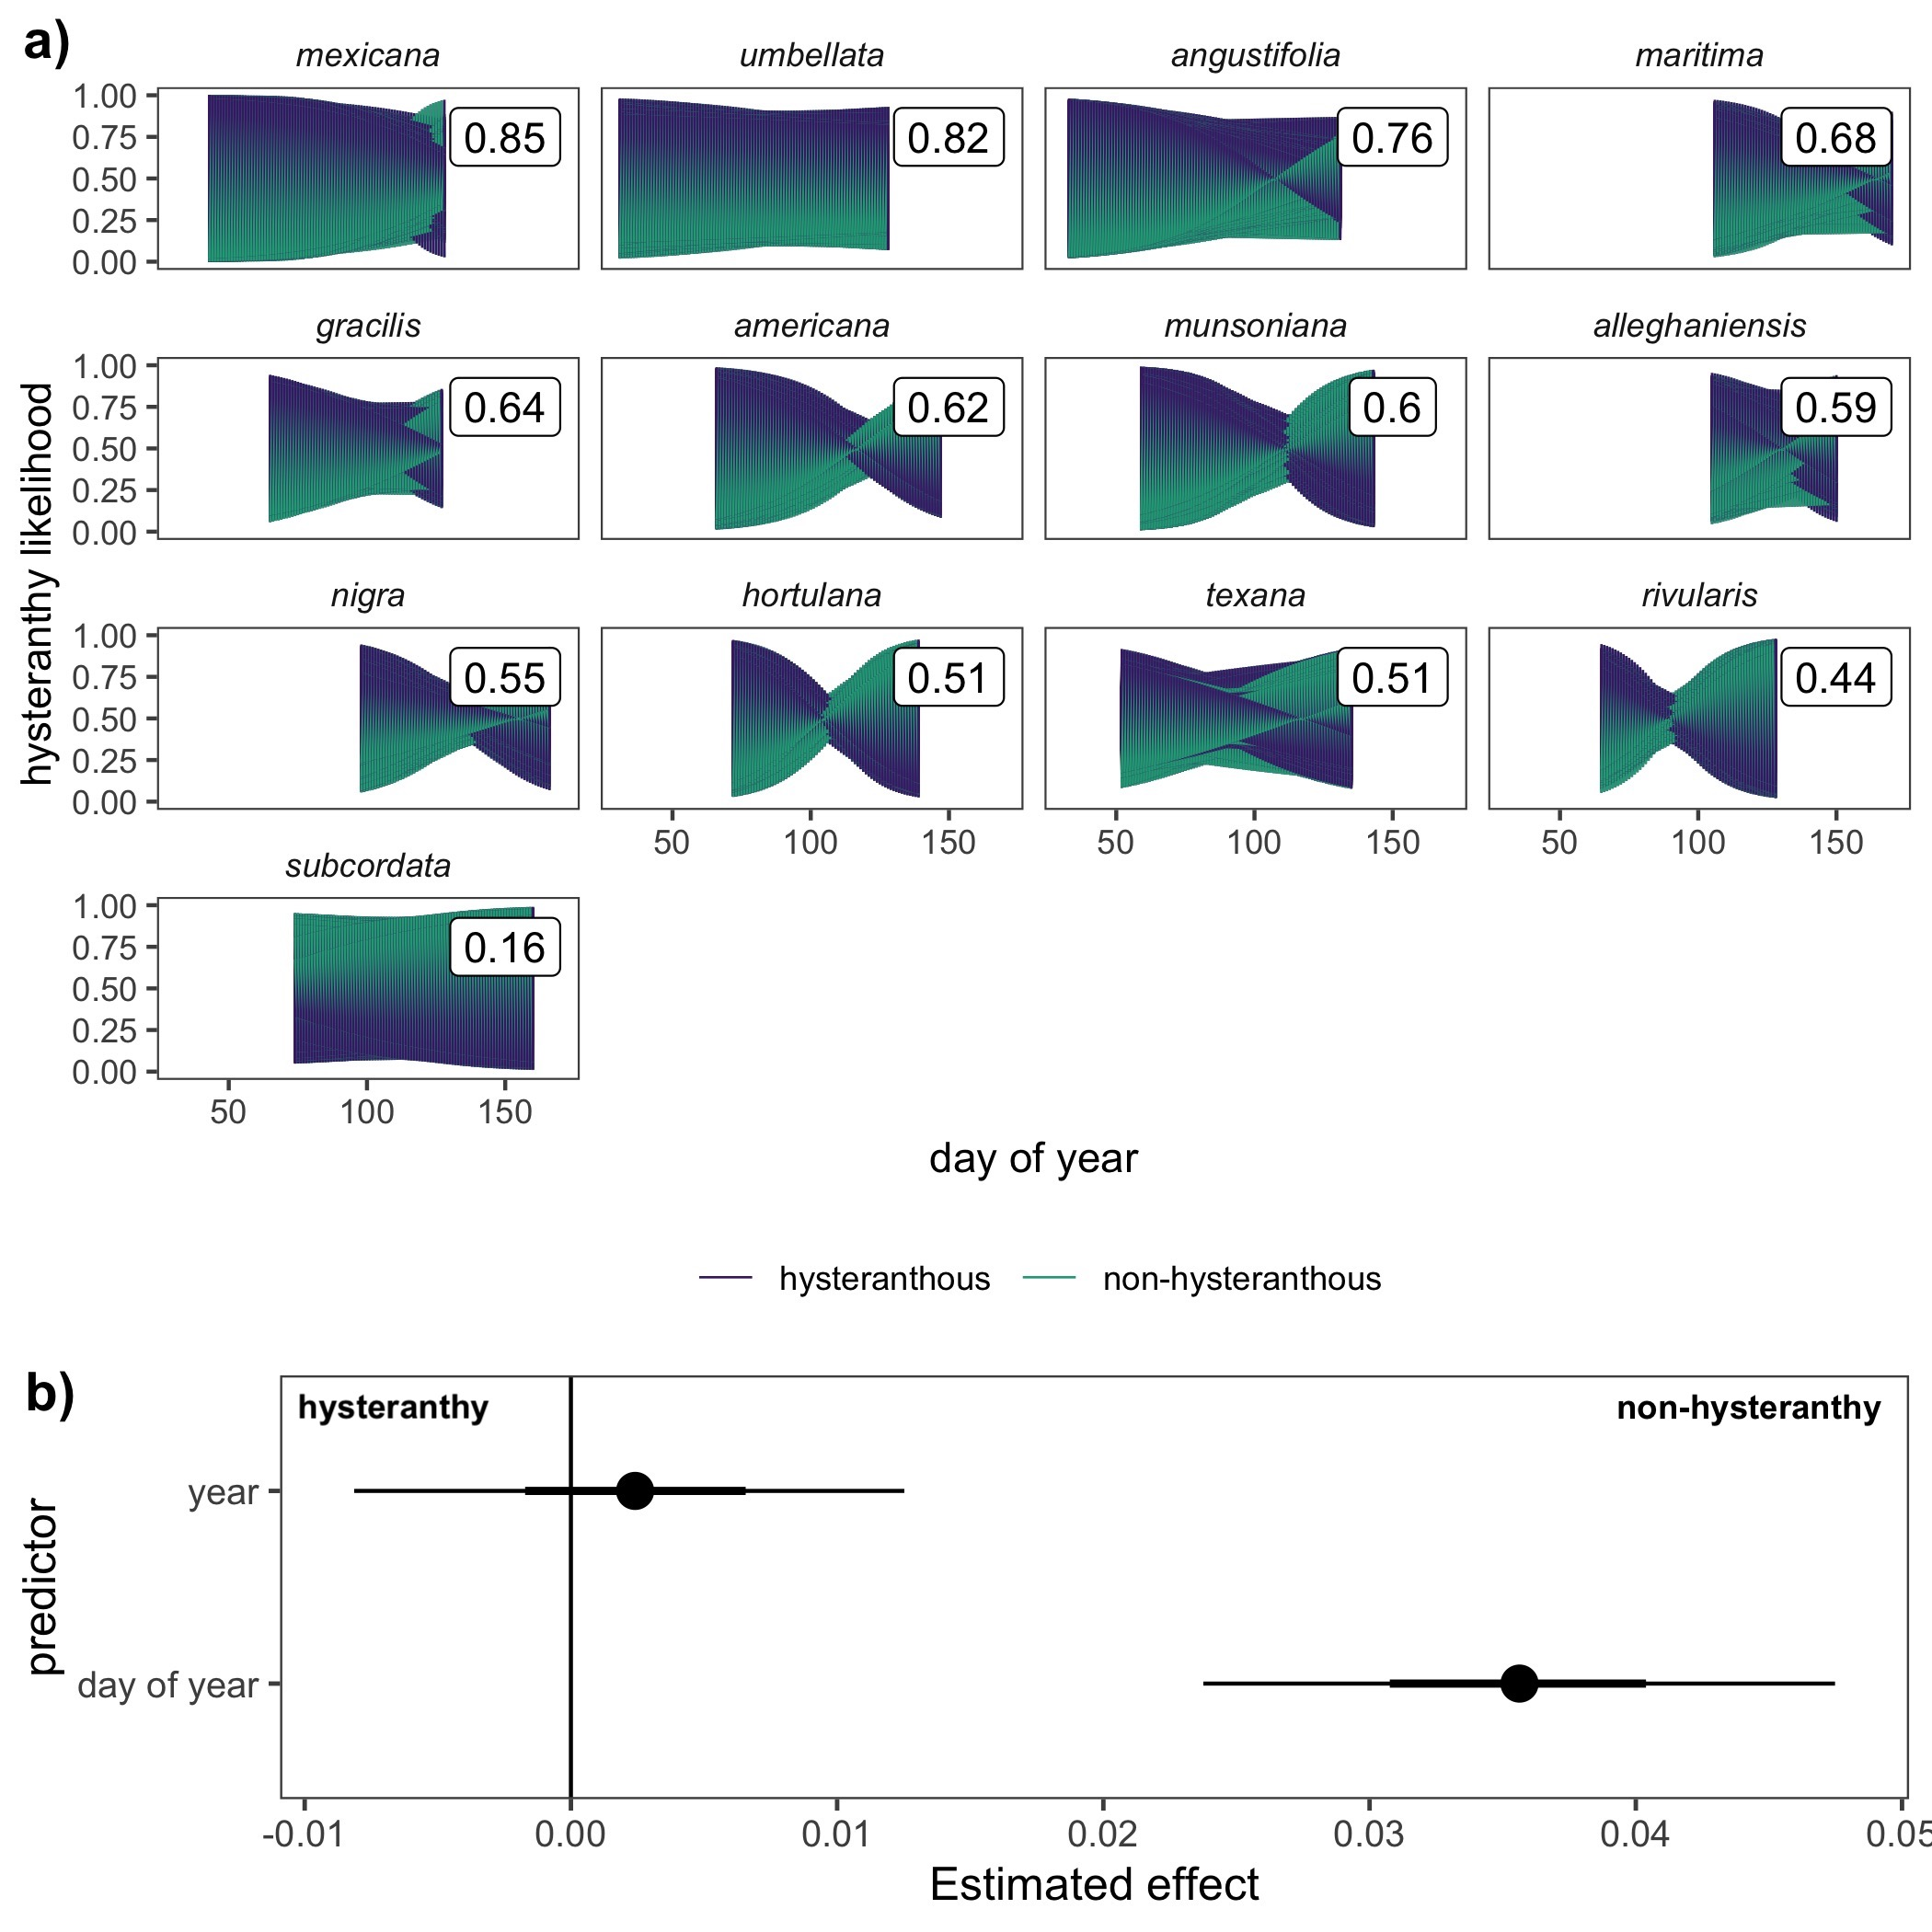
\includegraphics[width=\textwidth]{..//..//Plots/whatReviwerswant/sps_preds.jpeg}  %emw22Oct -- I would come up with easier language for the main text and mirror it here as much as possible. Also you have a ton of typos and I am not sure you ever mention panel a?
    \caption{Predicted likelihood of hysteranthy across the flowering period of 13 American plum species and the temporal predictors that drive these patterns. Panel a) depicts the predicted likelihood that each species would express hysteranthy on each day of their flowering season based on 1000 draws from the posterior distribution of Bayesian hierarchical models. The colored shapes represent how the likelihood changes over time and the boxed numerical values represent the average likelihood a species would express hysteranthy, summed across the full flowering period. % We defined hysteranthy as having open flowers at BBCH 0-BBCH 11 (leaf buds closed-start of leaf unfolding). See Tab. \ref{tab:mod1comps} for comparisons between the hysteranthous index scores reported here and alternative modeling approaches. }
    Panel b) depicts the influence of among season (year of sample) and within season (day of year of sample) trends on the likelihood species would express hysteranthy. Points are the mean effect size estimates, while thick and thin bars represent the 50\% and 89\% uncertainty intervals respectively.} 
    

    \label{fig:ordinals}
\end{figure}




\begin{figure}[h!]
    \centering
 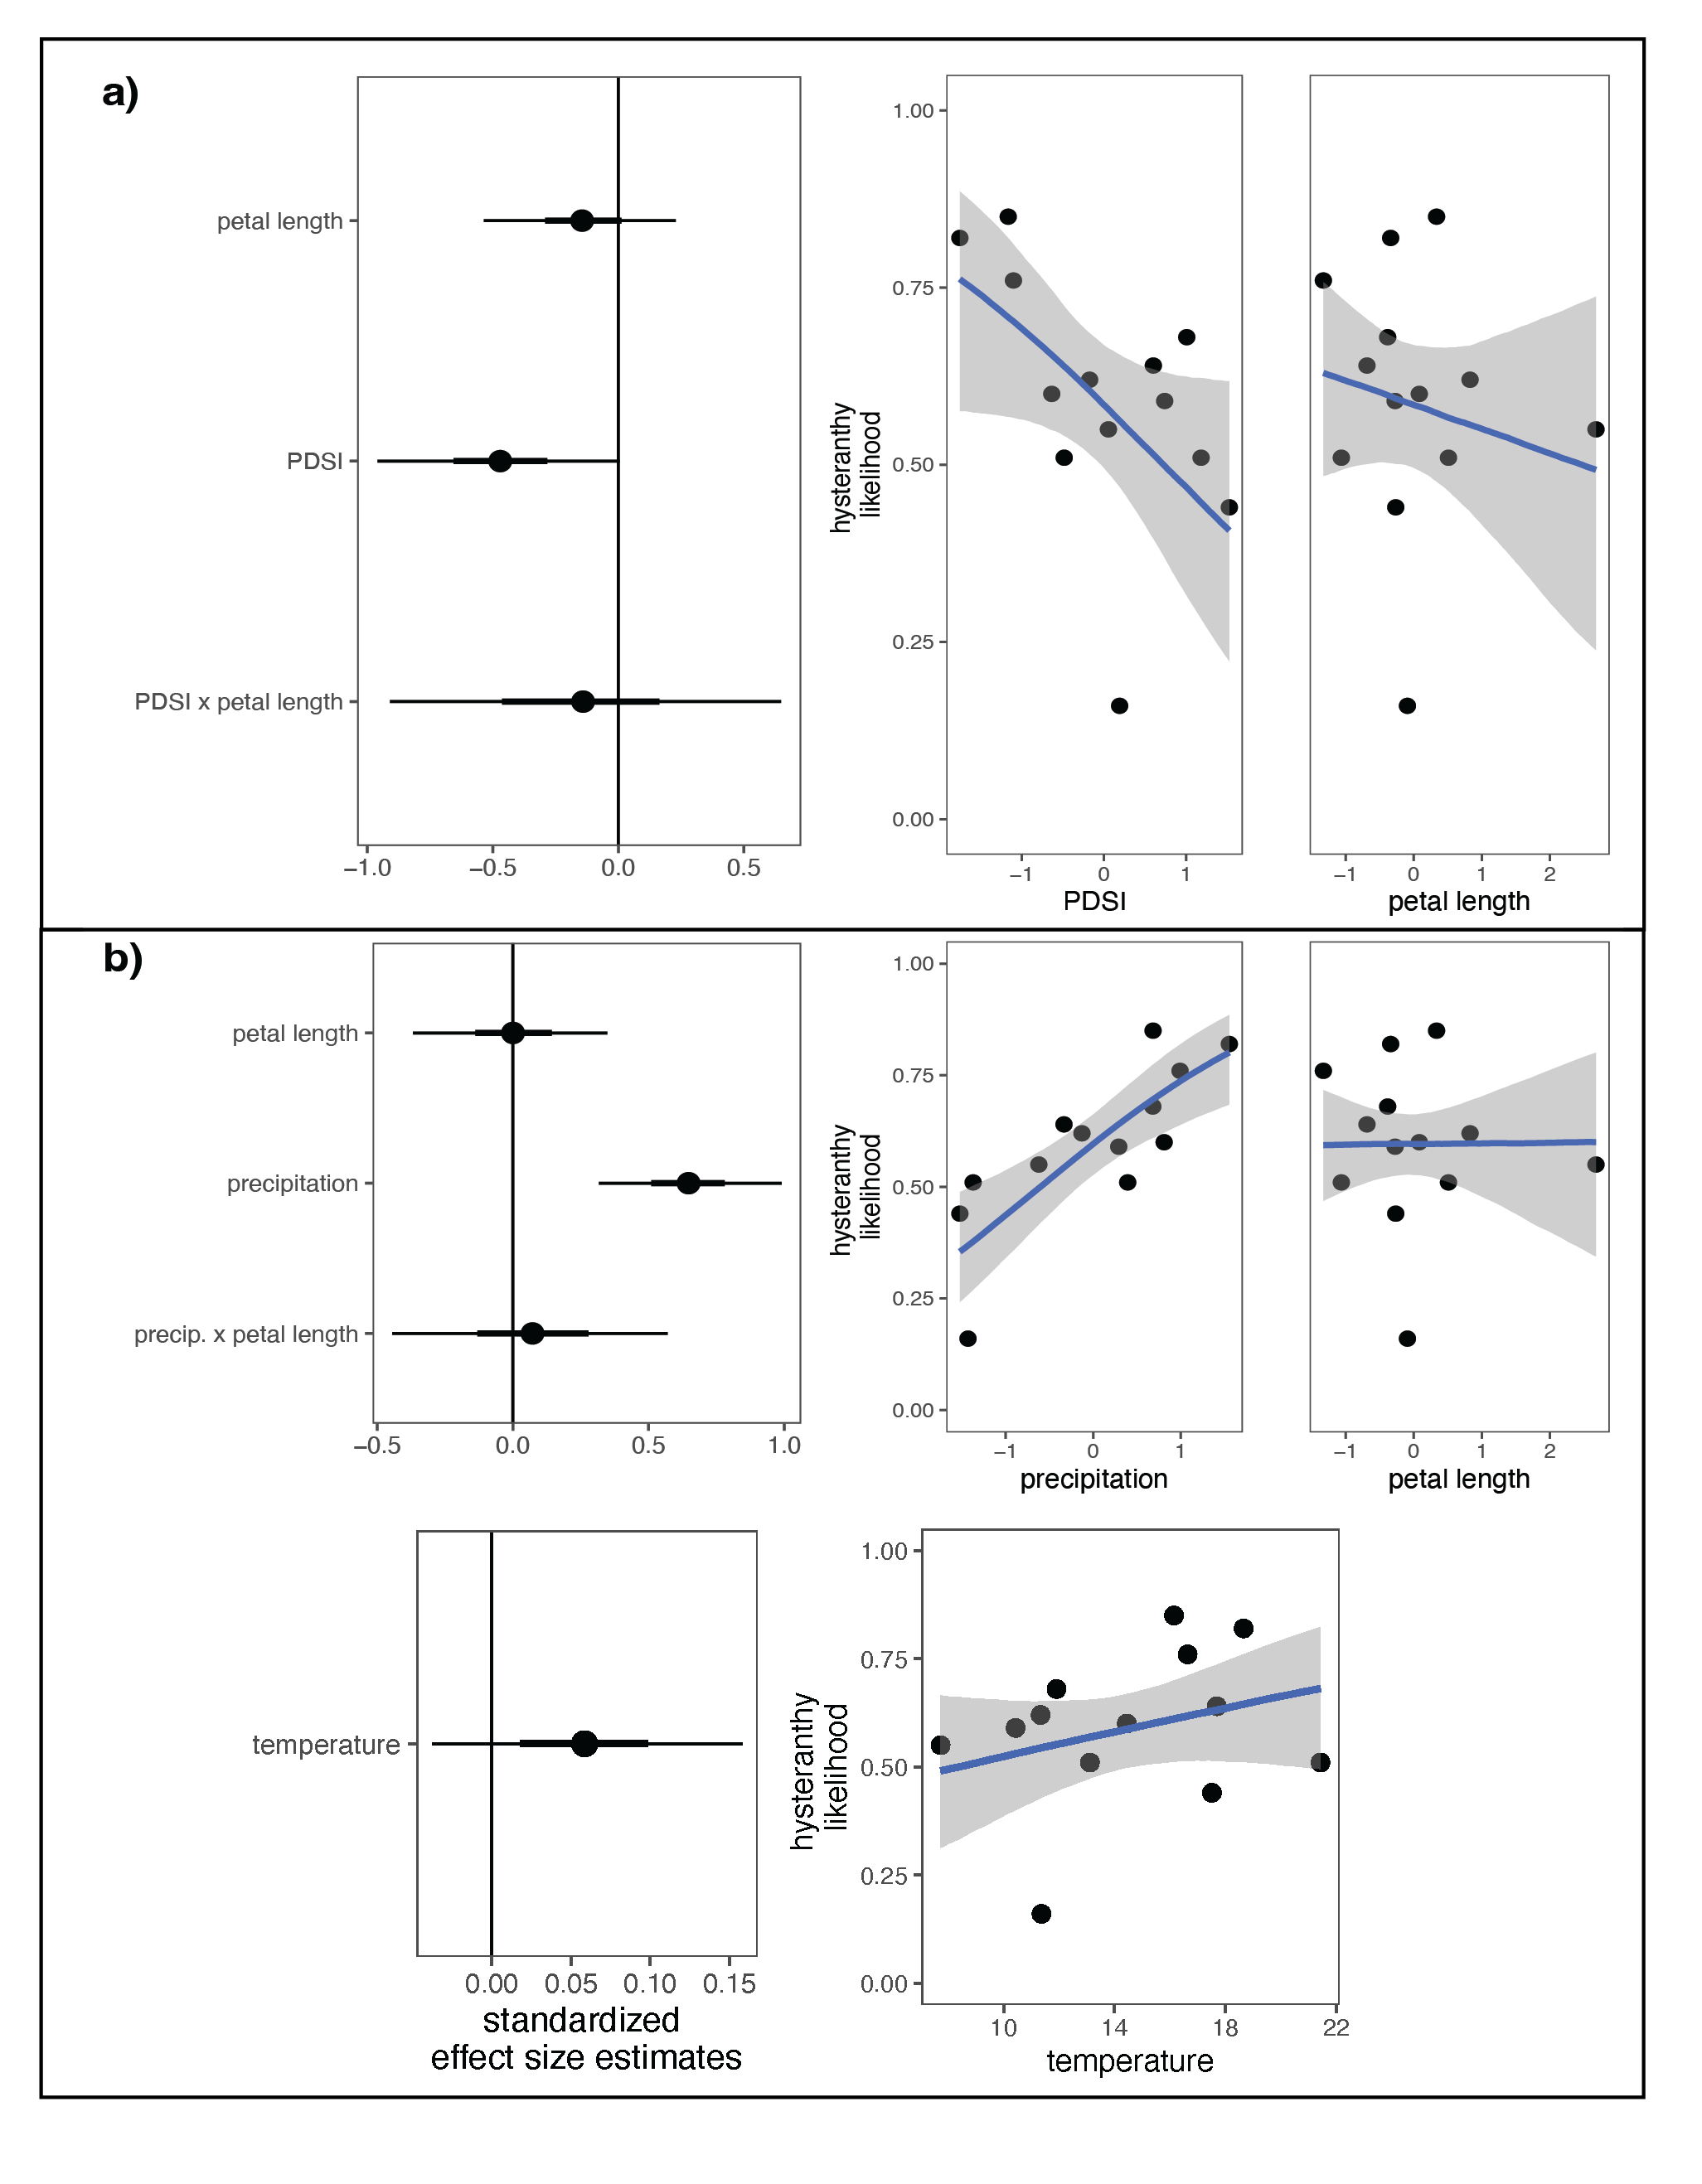
\includegraphics[width=.95\textwidth]{..//..//Plots/investfig3-01.png}
    \caption{Relationships between hysteranthy and environmental and biological traits for the 13 species of the American Plums. Panel a) shows the estimated effects of pdsi, petal length and their interaction on the likelihood hysteranthy. In the left plot points indicate the mean effects and the thick and thin bars represent the 50\% and 89\% uncertainty intervals, respectively. The right plots depict the conditional effects of each predictor on hysteranthy likelihood. Blue lines indicate the mean estimate and grey fill the 89\% uncertainty intervals. Predictor values ($x$-axis) have been $z$-scored to allow direct comparisons between predictors. Panel b) shows the same estimated effects but from models estimating the effects of mean annual precipitation, petal length and their interaction on the likelihood of hysteranthy, and the effects of mean annual temperature on hysteranthy.}
    \label{fig:prunes}
\end{figure}


\begin{figure}[h!]
    \centering
 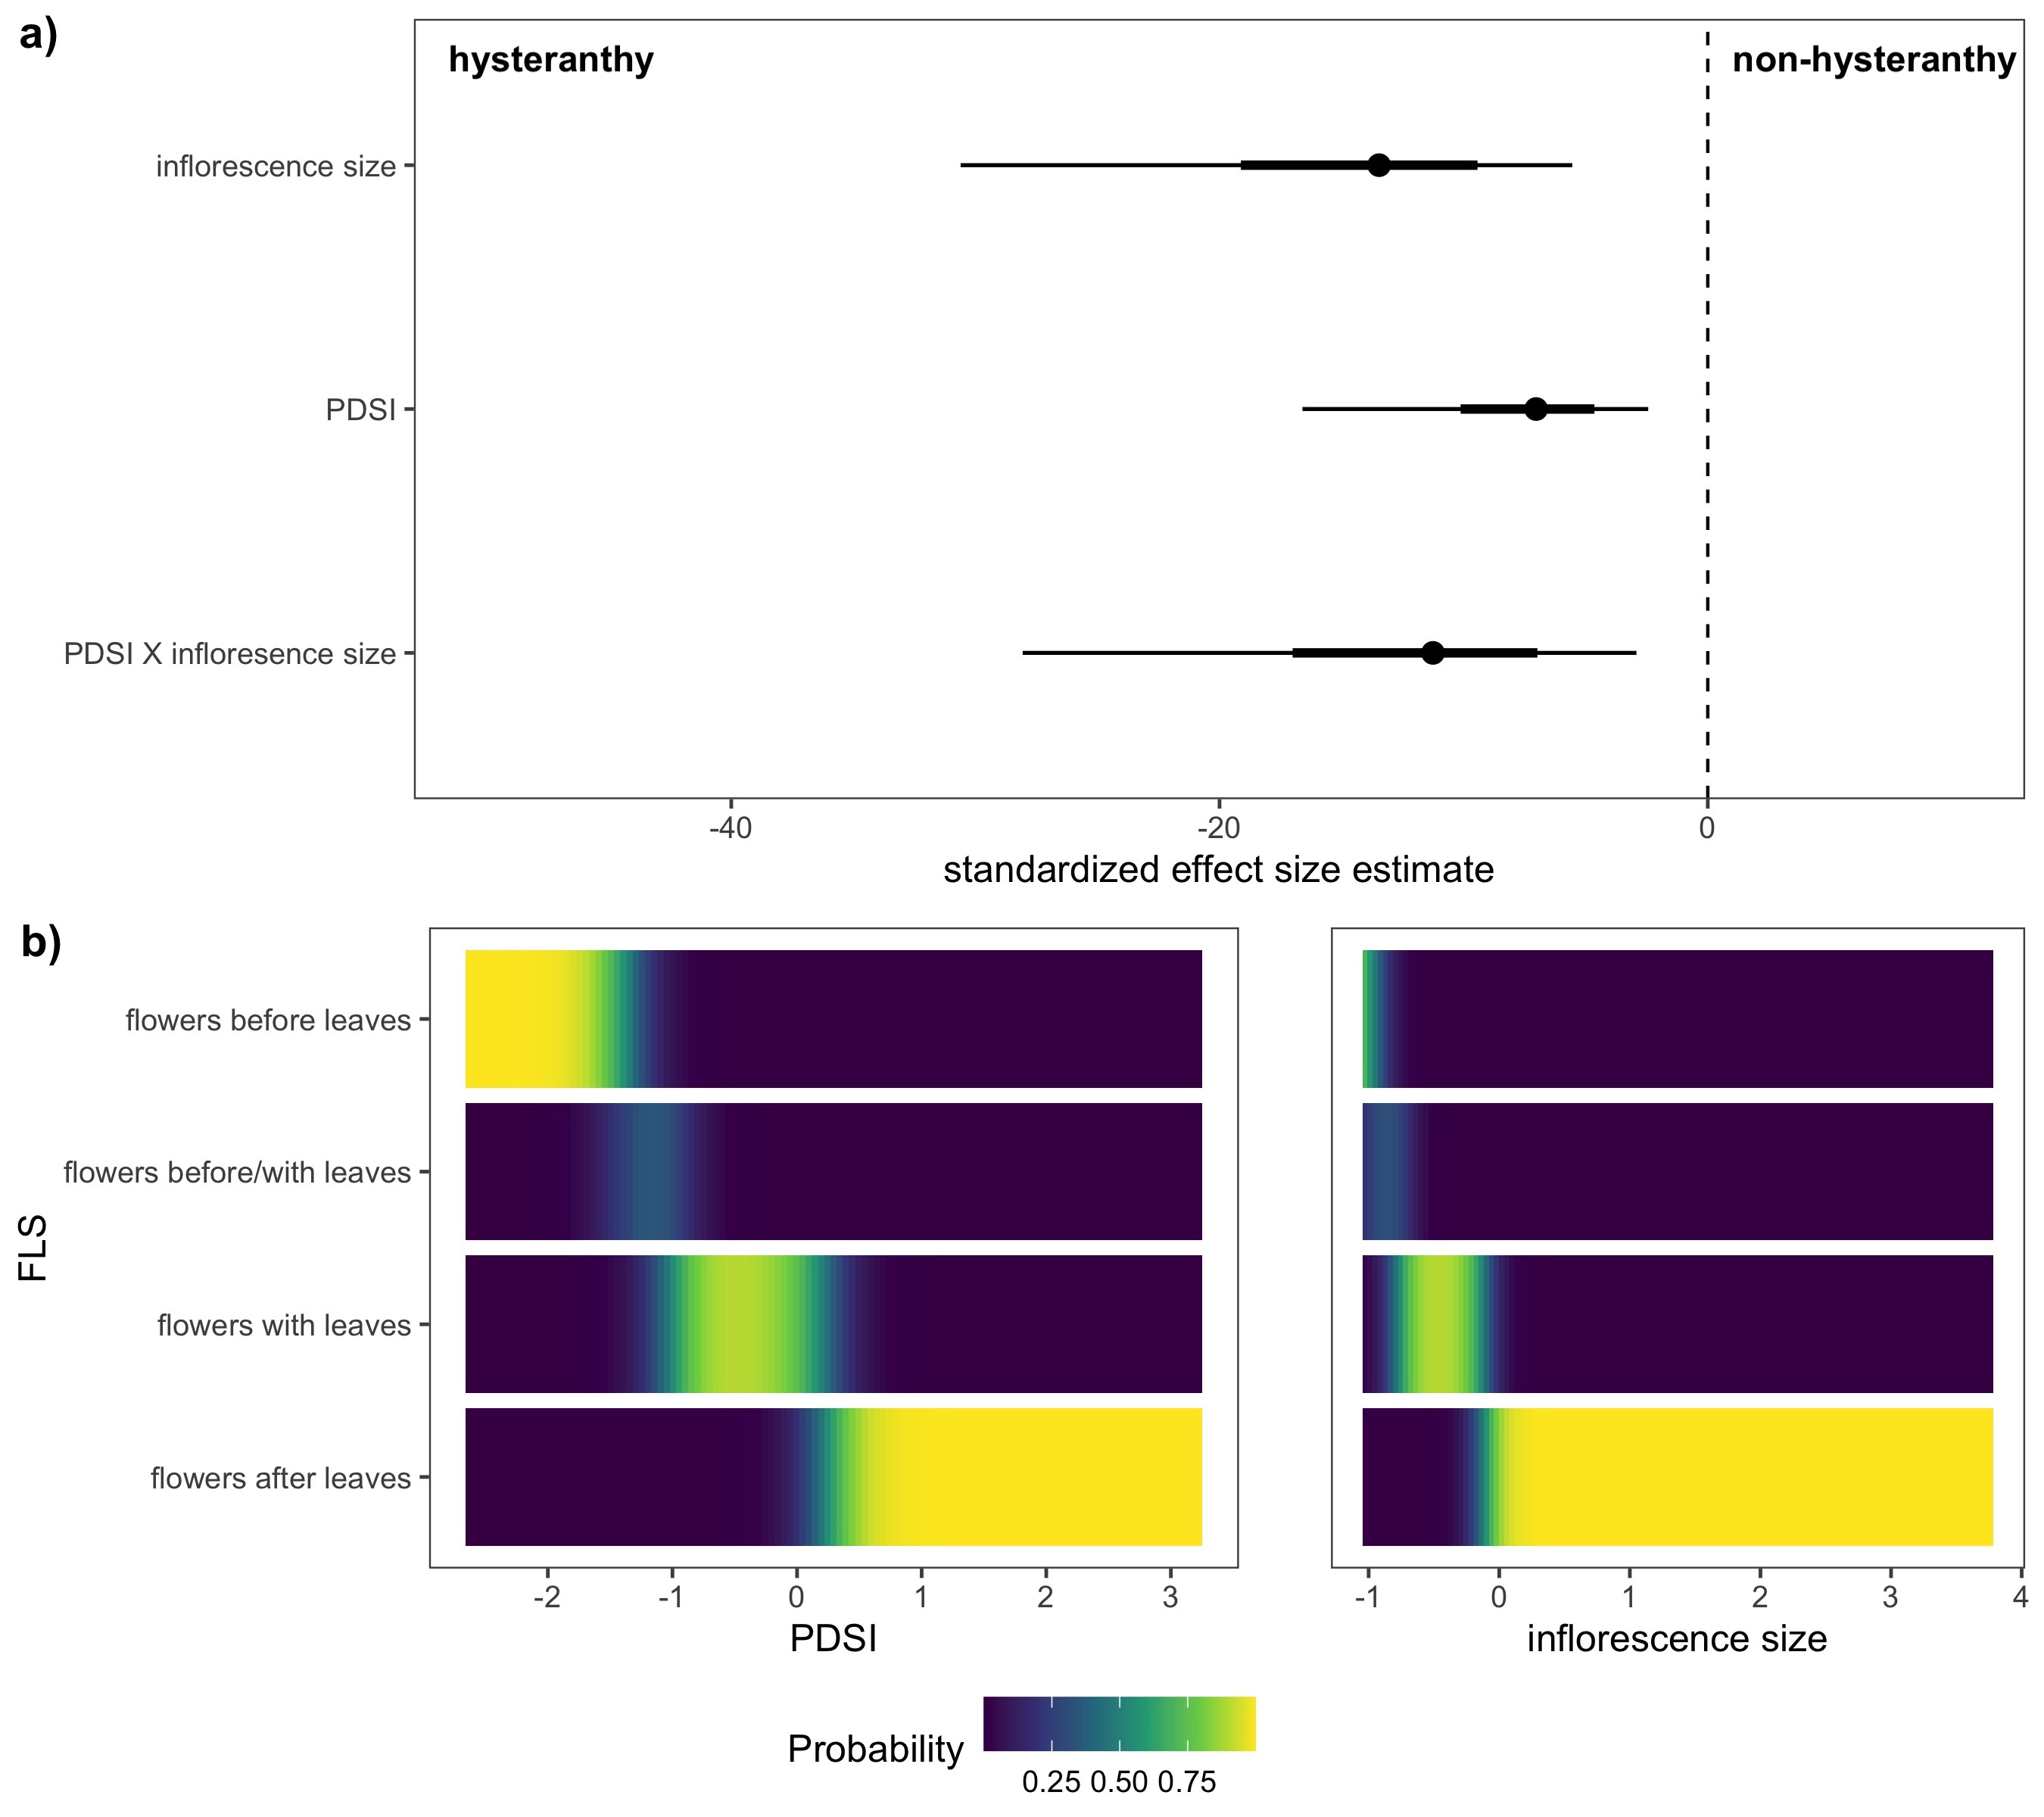
\includegraphics[width=\textwidth]{..//..//Plots/whatReviwerswant/fullprunus_4manu.jpeg} %emwmar9 --mv fruit to supp?
  %emw22Oct --  I like b! Could you make the conceptual order of (a) similar to previous figure? You have something about PDSI and floral display in both, keep the order the same for readers to see they are similar results. 
    \caption{Relationships between the likelihood of hysteranthy and environmental and biological traits for 32 species of the genus \emph{Prunus} native to, or established in North America. Panel a) shows the estimated effect size of each predictor. Points indicate the mean estimate for each predictor, and thick and thin bars the 50\% and 89\% uncertainty intervals, respectively. Panel b) depicts the likelihood for each flower-leaf sequence stage ($y$-axis) at any given values of PDSI or number of flowers/inflorescence (inflorescence size). Predictor values ($x$-axis) have been $z$-scored to allow direct comparisons between predictors.}
    \label{fig:genus}
\end{figure}

\begin{figure}[h!]
    \centering
 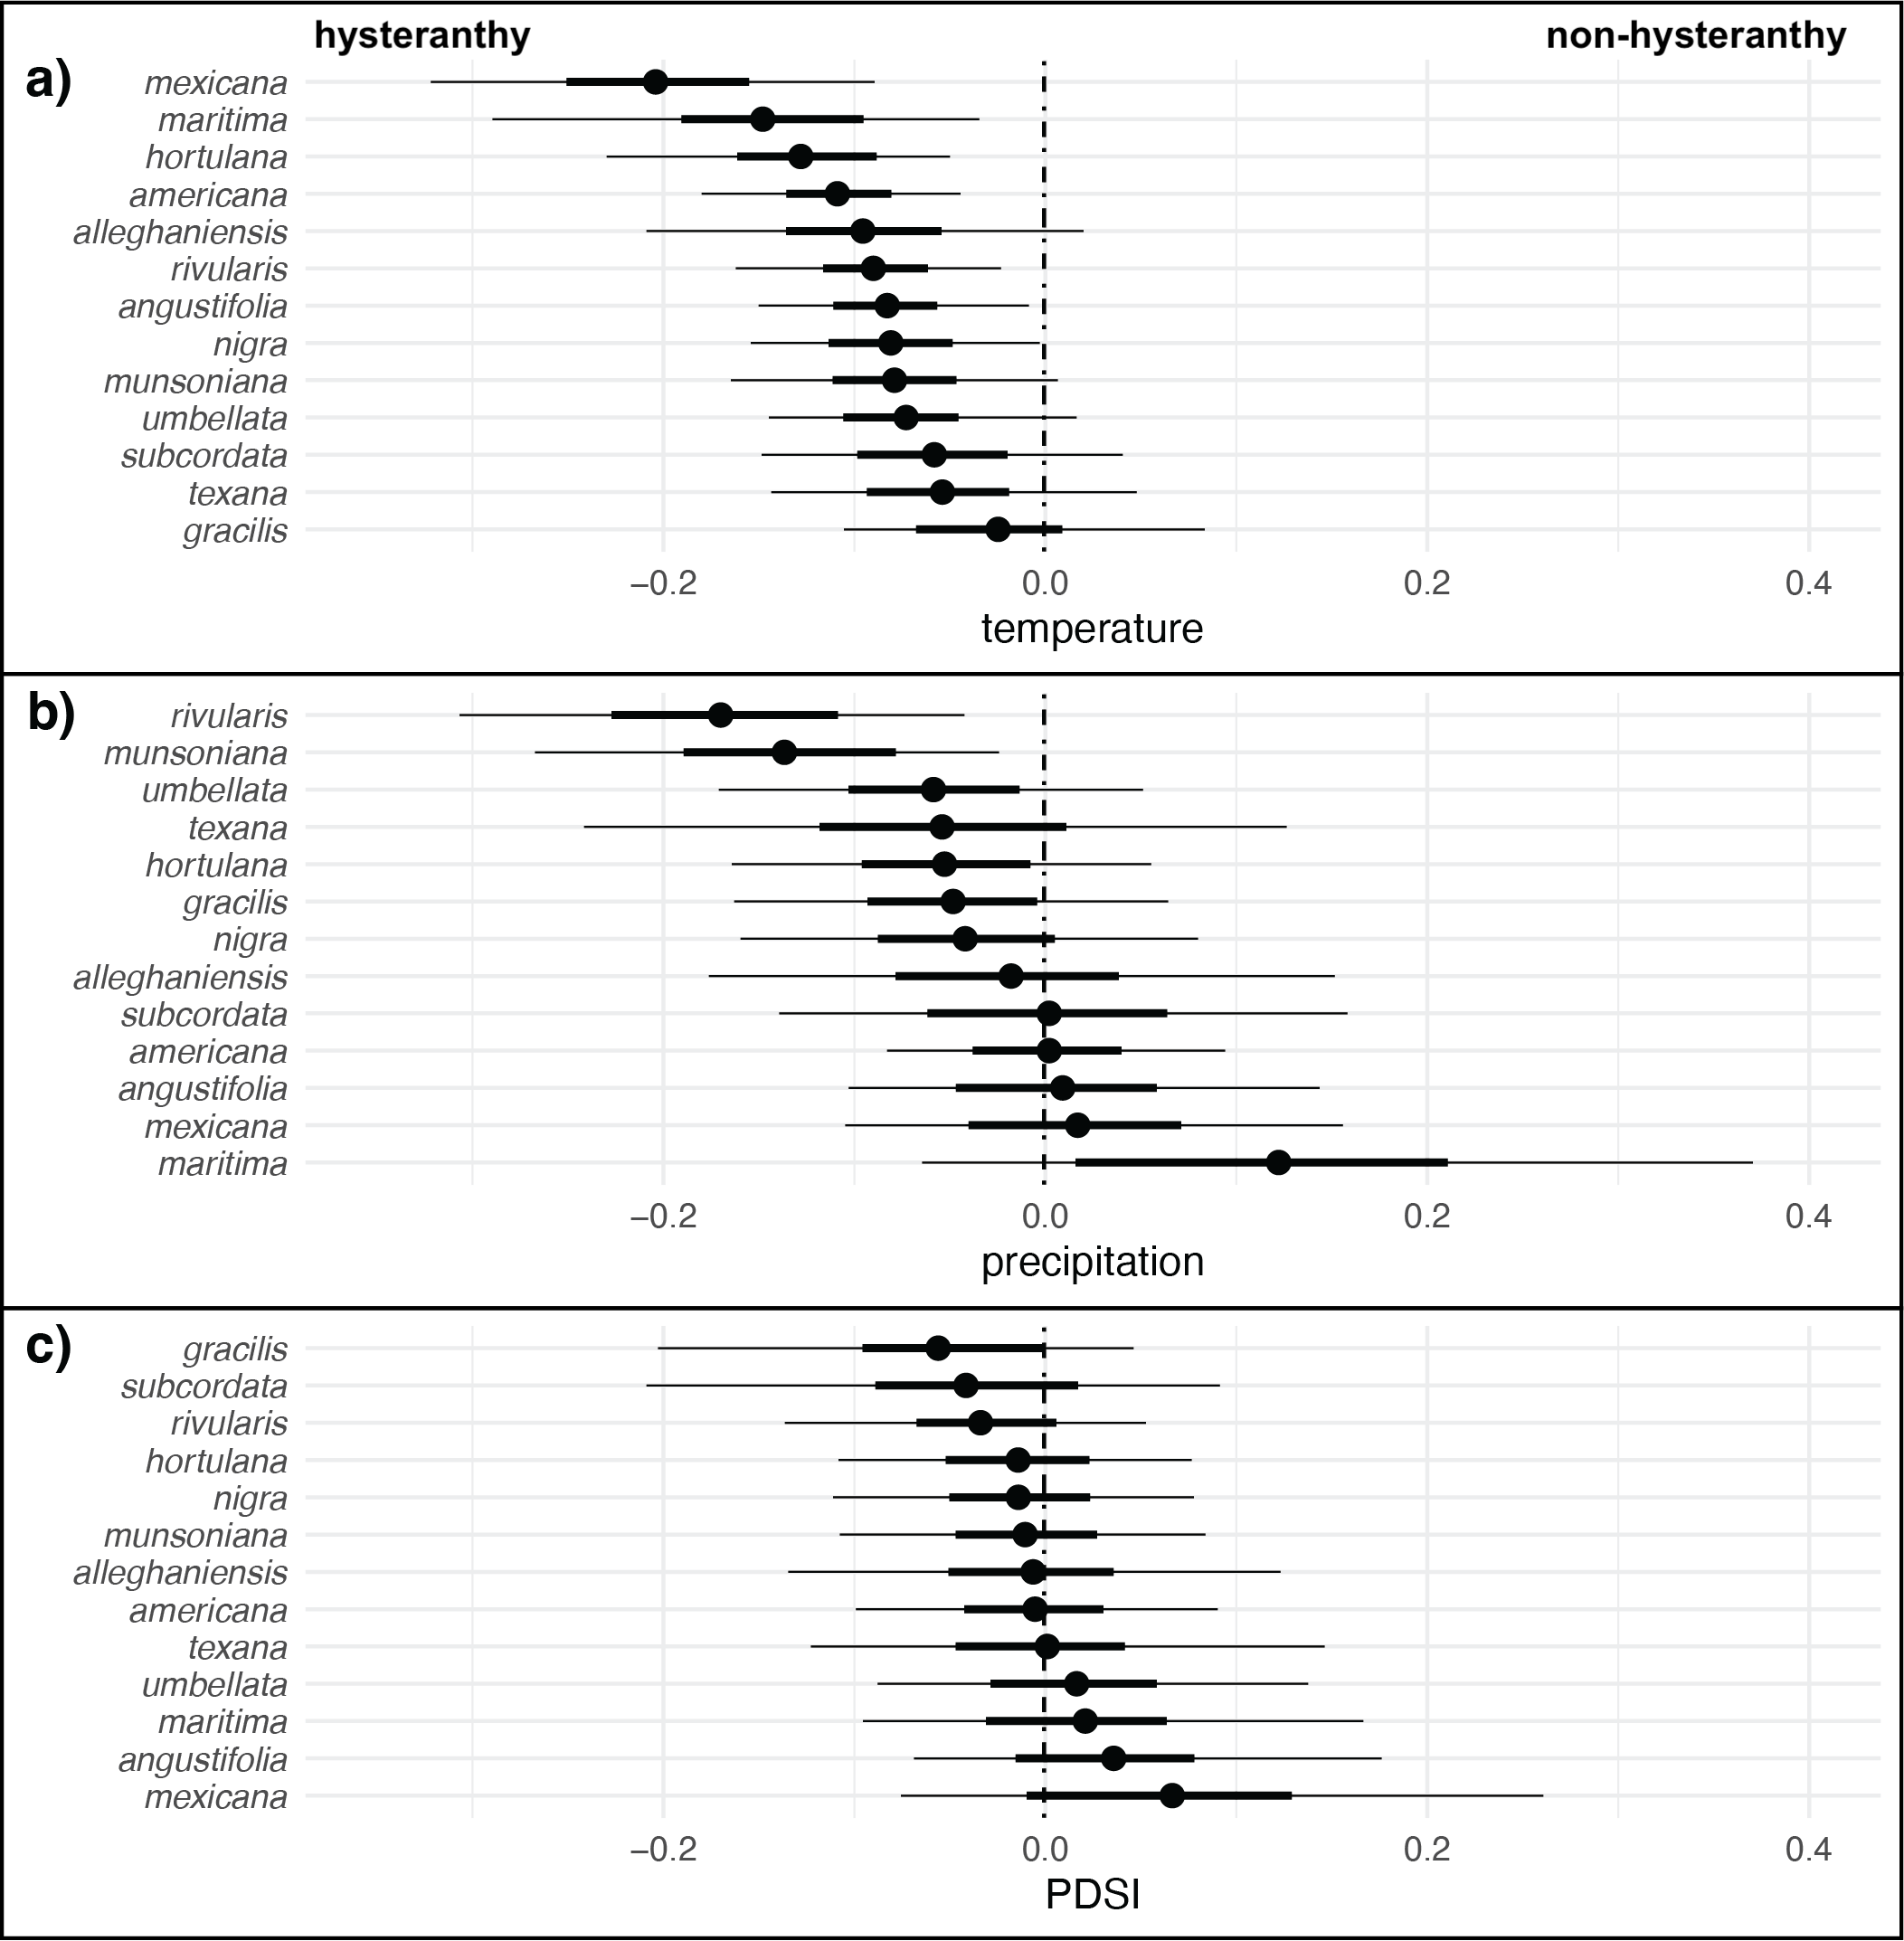
\includegraphics[width=\textwidth]{..//..//Plots/plasticity.png} %emwmar9 --mv fruit to supp?
  %emw22Oct --  I like b! Could you make the conceptual order of (a) similar to previous figure? You have something about PDSI and floral display in both, keep the order the same for readers to see they are similar results. 
    \caption{Effects of climate variables on intraspecific variation in flower-leaf sequences. Panel a) displays the effect of annual temperature, panel b) the effect of annual precipitation and pannel c) annual PDSI.  Points indicate the mean effects and the thick and thin bars represent the 50\% and 89\% uncertainty intervals, respectively.}
    \label{fig:plastic}
\end{figure}


\end{document}
